\chapter{Control System and Automation}

\section{Introduction}
This chapter will detail the automation logic and programming of the robotic sorting cell. It will cover the overall control philosophy, the programming environment, and the specific implementation details for the PLC and HMI.

\section{General Overview}
The control of the robotic sorting cell is handled by a Programmable Logic Controller (PLC), which acts as the central brain of the system. The PLC was chosen for its reliability, real-time processing capabilities, and industrial robustness. It continuously monitors the state of all sensors and, based on a pre-defined logic, sends commands to the actuators. The control philosophy prioritizes safety, sequential operation, and synchronization between all components, including the KUKA robot, conveyors, and pneumatic cylinders. This structured approach is fundamental to the system's efficient and predictable behavior.


\section{PLC Programming and Implementation}
This section details the programming of the PLC, covering the initial configuration, tag management, and the development of the main control logic.

\subsection{Hardware and Network Configuration}
The hardware and network configuration is the foundational step in a TIA Portal project, where the physical components are digitally modeled, and their communication links are established. This process ensures that all devices can interact seamlessly, forming a cohesive automation system. To make this process as clear as possible, it is broken down into a series of logical steps.

\begin{itemize}
\item Step 1: Component Selection

The first step involves selecting the appropriate hardware from TIA Portal's catalog, as shown in Annex \ref{fig:plc_selection} and Annex \ref{fig:hmi_selection}. This project utilized a physical SIMATIC S7-1212C PLC for the final application. However, for all simulation and virtual commissioning, a more advanced SIMATIC S7-1513-1 PN PLC was selected due to the requirements of the S7-PLCSIM Advanced software. This distinction between the physical and virtual hardware is crucial for a complete understanding of the development process. Additionally, the Human-Machine Interface (HMI) panel, which serves as the operator's primary control point, was also selected from the catalog to provide the necessary screen size and functionality for the sorting cell's interface. Specifically, the SIMATIC Unified Comfort Panel (MTP1200 Unified Comfort) was chosen;


\item Step 2: Network Setup

Once the devices (PLC and HMI) were added to the project, the network view within TIA Portal was used to establish communication links. This graphical interface allows for the virtual connection of devices, creating a logical representation of the physical network. The devices were interconnected via industrial Ethernet, which serves as the backbone for data exchange using the S7 communication protocol. The network topology is shown in Figure \ref{fig:network_setup};
\begin{figure}[H]
    \centering
    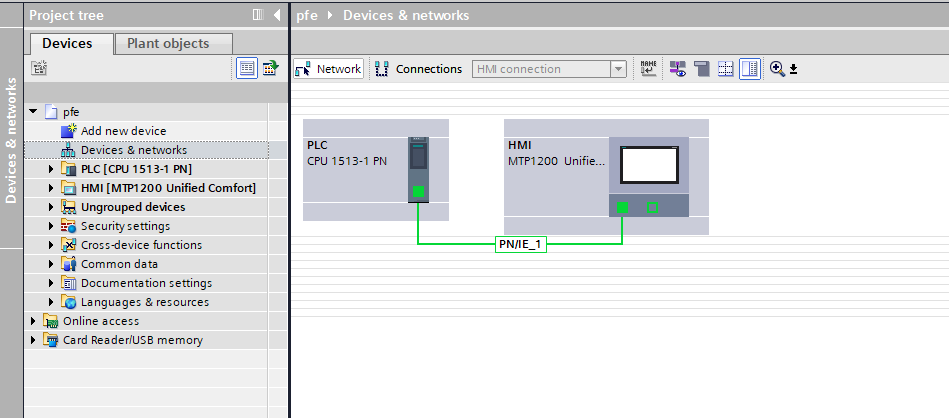
\includegraphics[width=0.9\textwidth]{Images/Chap3/connection.png}
    \caption{Network topology showing communication links between the PLC and HMI.}
    \label{fig:network_setup}
\end{figure}

\item Step 3: IP Address Configuration

A robust and reliable network is dependent on a consistent IP address schema. In this step, a unique IP address and a common subnet mask were assigned to each device to ensure seamless communication. The physical PLC was assigned the address 192.168.0.1 and the HMI was set to 192.168.0.2. The subnet mask for all devices was configured as 255.255.255.0, establishing that they all reside on the same network segment and can exchange data without any routing issues. The IP address configuration for network devices is shown in Figure \ref{fig:ip_configuration}.
\begin{figure}[H]
    \centering
    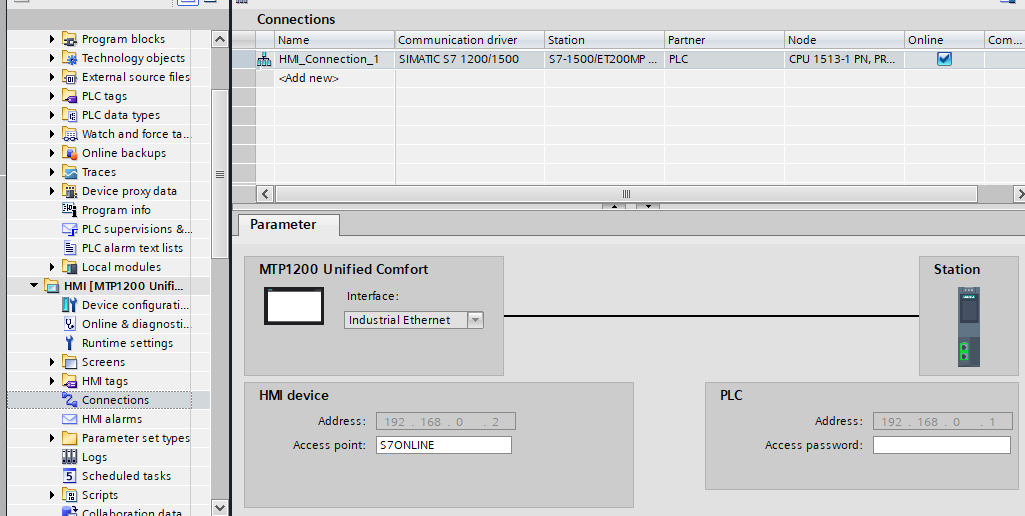
\includegraphics[width=0.9\textwidth]{Images/Chap3/Ips.png}
    \caption{IP address configuration for network devices.}
    \label{fig:ip_configuration}
\end{figure}

\end{itemize}

\subsection{Data Management and Tagging}
Effective data management is crucial for a well-structured and maintainable program. All I/O signals and internal variables are organized into Data Blocks (DBs) for a clear and logical structure.

\subsubsection{Input and Output Tags}
All physical inputs and outputs are mapped to their corresponding addresses in a dedicated InputDB and OutputDB, as shown in Figure \ref{fig:input_tags} and Figure \ref{fig:output_tags}. This makes the program hardware-independent, as the main logic can reference these tags without being directly tied to physical addresses.
\begin{figure}[H]
\centering
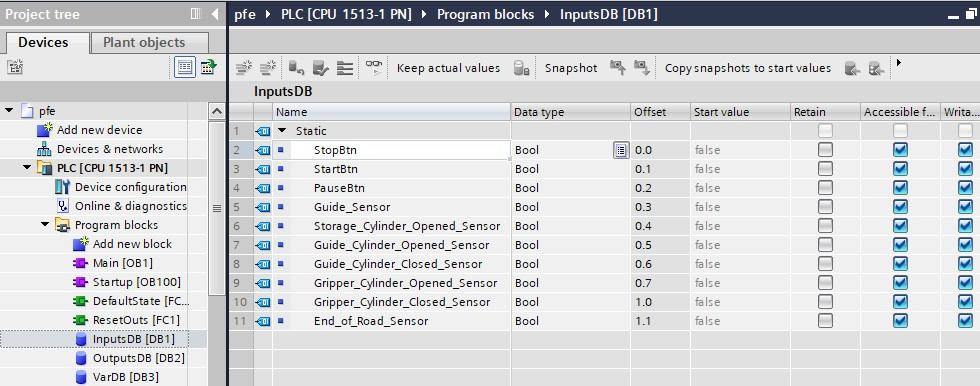
\includegraphics[width=1\textwidth]{Images/Chap3/tags_inputs_db.jpg}
\caption{Mapping physical inputs to symbolic tags.}
\label{fig:input_tags}
\end{figure}
\begin{figure}[H]
\centering
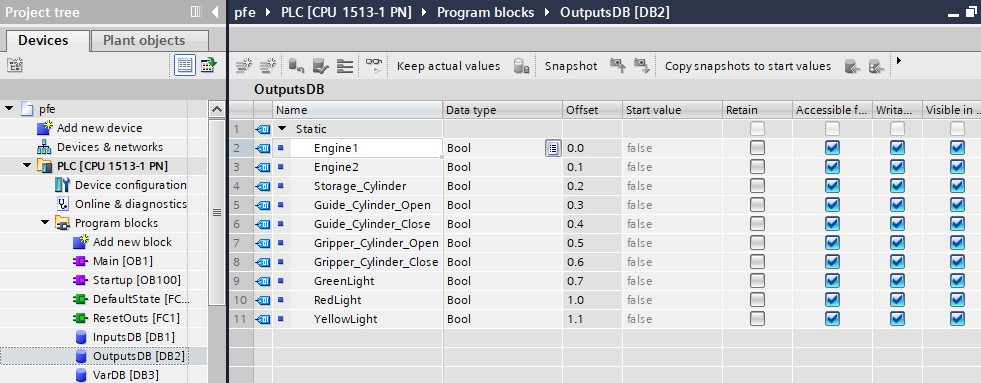
\includegraphics[width=1\textwidth]{Images/Chap3/tags_outputs_db.jpg}
\caption{Mapping physical outputs to symbolic tags.}
\label{fig:output_tags}
\end{figure}

\subsubsection{Internal tags}
A key part of this structured approach was the use of a dedicated set of internal tags, from \textbf{X0 to X13}, to track the active steps of the GRAFCET sequence. This direct mapping between the GRAFCET steps and the PLC tags made the implementation of the sequential logic straightforward and easy to debug.

The following figure provides a visual overview of the tag management for the GRAFCET steps, showing their direct mapping to the sequential logic.
\begin{figure}[H]
    \centering
    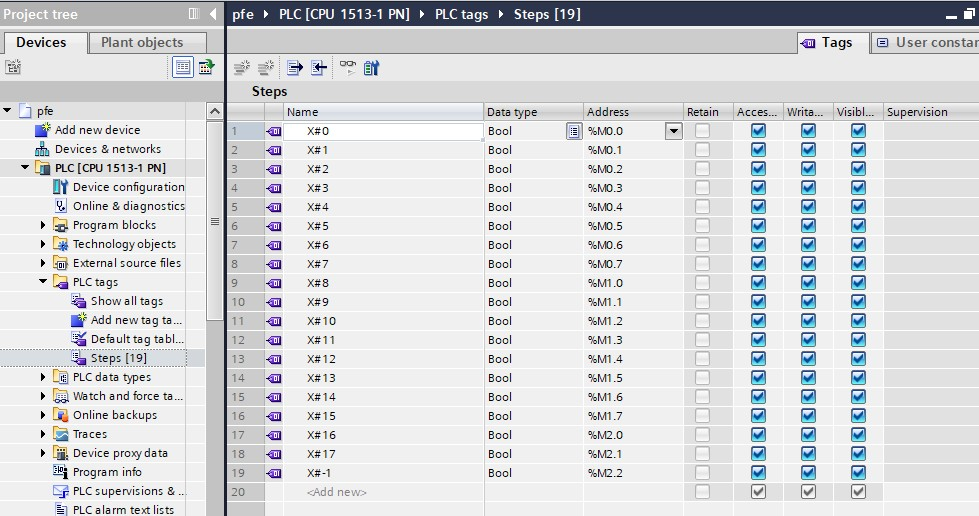
\includegraphics[width=1\textwidth]{Images/Chap3/tags_steps.jpg}
    \caption{TIA Portal screenshot showing the tags for the GRAFCET steps (X0-13).}
    \label{fig:tags_steps}
\end{figure}
\subsubsection{State Variables}
This section defines the key internal state variables used by the program. These variables are stored in a dedicated Global Data Block (VarDB), which allows them to be accessed from any part of the program. They include the operational status, sequential steps, and actuator control variables, as detailed below:

\begin{itemize}
\item Status Variable (VarDB.Status)
This variable controls the overall operational mode of the cell, dictating its behavior during the cycle.
\begin{table}[H]
    \centering
    \begin{tabular}{|p{0.15\textwidth}|p{0.35\textwidth}|}
        \hline
        \textbf{Value} & \textbf{State Description} \\
        \hline
        
        0 & Stop Mode \\
        \hline
        1 & Running Mode \\
        \hline
        2 & Pause Mode \\
        \hline
        3 & Maintenance Mode \\
        \hline
        4 & Resetting Mode \\
        \hline
    \end{tabular}
\end{table}

\item Robot Status Variable (VarDB.RobotStatus)
This variable indicates the current status of the KUKA robot, allowing the PLC to know if the robot is waiting or moving.
\begin{table}[H]
    \centering
    \begin{tabular}{|p{0.15\textwidth}|p{0.35\textwidth}|}
        \hline
        \textbf{Value} & \textbf{State Description} \\
        \hline
        0 & At Home Position \\
        \hline
        1 & Moving \\
        \hline
        2 & Ready \\
        \hline
        3 & Paused \\
        \hline
    \end{tabular}
\end{table}

\item Robot Position Variable (VarDB.RobotPos)
An integer value that sends the robot to a specific position. The PLC sends one of these values to the robot to command it to move to a defined location.
\begin{table}[H]
    \centering
    \begin{tabular}{|p{0.15\textwidth}|p{0.35\textwidth}|}
        \hline
        \textbf{Value} & \textbf{State Description} \\
        \hline
        0 & Home Position \\
        \hline
        1 & Pick-up Position \\
        \hline
        2 & Red Bin Position \\
        \hline
        3 & Green Bin Position \\
        \hline
        4 & Blue Bin Position \\
        \hline
    \end{tabular}
\end{table}

\item Cube Color Variable (VarDB.CubeColor)
This integer value represents the color of the cube detected by the vision system, a key input for the sorting logic, and is set by the Raspberry Pi after it processes the vision data.
\begin{table}[H]
    \centering
    \begin{tabular}{|p{0.15\textwidth}|p{0.35\textwidth}|}
        \hline
        \textbf{Value} & \textbf{State Description} \\
        \hline
        1 & Red Cube \\
        \hline
        2 & Green Cube \\
        \hline
        3 & Blue Cube \\
        \hline
        0 & No Cube Detected \\
        \hline
    \end{tabular}
\end{table}

\item Cylinder Control Variables (VarDB.GuideState / VarDB.GripperState)
These variables control the pneumatic cylinders, which are used to guide the cubes and operate the gripper. They share a similar logic where an integer value dictates the state of the actuator.

   \begin{table}[H]
        \centering
        \begin{tabular}{|p{0.15\textwidth}|p{0.35\textwidth}|}
            \hline
            \textbf{Value} & \textbf{State Description} \\
            \hline
            1 & Idle \\
            \hline
            2 & Open Cylinder \\
            \hline
            4 & Close Cylinder \\
            \hline
        \end{tabular}
    \end{table}

\item Cube Counter Variables
These integer variables are used to track the number of cubes sorted, providing essential feedback on the system's performance.
\begin{itemize}
    \item VarDB.BlueCubesCounter
    \item VarDB.GreenCubesCounter
    \item VarDB.RedCubesCounter
\end{itemize}

\end{itemize}

The main state variables defined in the Global Data Block are shown in Figure \ref{fig:tags}.
\begin{figure}[H]
\centering
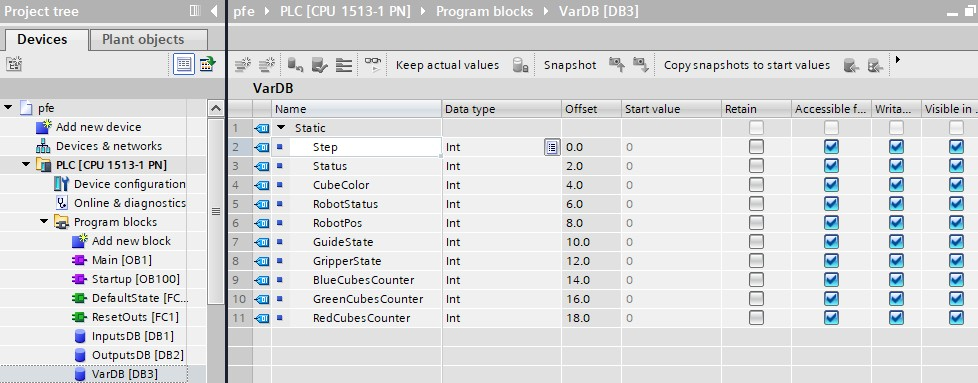
\includegraphics[width=1\textwidth]{Images/Chap3/tags_variables_db.jpg}
\caption{The main state variables defined in the Global Data Block.}
\label{fig:tags}
\end{figure}


\subsection{GRAFCET}
To design and visualize the sequential control logic, a GRAFCET (Graph for Step-by-Step Control) approach was used. GRAFCET is a graphical language that simplifies complex automation sequences by breaking the process down into a series of steps and transitions. Each step represents a state of the system where specific actions occur, while each transition defines the conditions that must be met to move to the next step.

Transitions between these steps are triggered by logical conditions, such as sensor signals confirming a part's presence, operator inputs from the HMI, or completion signals from the robotic arm. This method ensures a clear, visual representation of the entire process, making it easy to understand, debug, and modify the control logic.

The final GRAFCET, as shown in Annex \ref{fig:grafcet_logic}, was designed to manage a single, complete sorting cycle. This design decision, while limiting continuous operation, was necessary due to the constraints of the simulation environment, where automated sensor activation for a continuous loop could not be realistically emulated. The diagram presents the primary operational sequence, which handles the sorting process from start to finish. A 3D representation of the automated sorting cell with key components is also shown in Annex \ref{fig:cell_3d_view_annotated}.



\subsection{Programming Languages and Fundamental Blocks}
For this project, the primary language used was Ladder Diagram (LAD). Its graphical, relay-logic format was ideal for implementing and troubleshooting the sequential control logic. Within LAD, the control logic is built using a combination of fundamental blocks. The following are the most important blocks used in this project:

\subsubsection{Comparison Blocks}

Functionality: These blocks are used to compare two values and return a Boolean result (TRUE or FALSE). They are essential for creating conditional logic within the program. The images show a comparison for both equality (==) and inequality (<>), as shown in Figure \ref{fig:comparison_blocks}.

Inputs and Outputs: Comparison blocks take two numerical inputs (e.g., from an integer variable or a constant value) and provide a single Boolean output.

When to Use: These blocks are used to check the status of a variable before allowing a specific action to proceed. For instance, comparing the CubeColor variable to a specific integer to determine the type of object, or checking the RobotStatus variable for a specific value to confirm the robot is ready.
\begin{figure}[H]
\centering
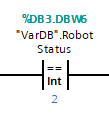
\includegraphics[width=0.2\textwidth]{Images/Chap3/tags_equals.png}
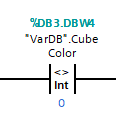
\includegraphics[width=0.2\textwidth]{Images/Chap3/tags_different.png}
\caption{Comparison blocks for equality and inequality.}
\label{fig:comparison_blocks}
\end{figure}

\subsubsection{Move Blocks}
Functionality: The MOVE block transfers the value from its input (IN) to its output (OUT). A typical MOVE block in Ladder Diagram is shown in Figure \ref{fig:move_block_lad}.

Inputs and Outputs: The input can be a numerical value, a constant, or a variable address. The output is a variable address where the value will be stored. The block also has a Boolean enable input (EN) and output (ENO) to control its execution.


When to Use: This block is used to set the value of a variable. A common application in this project is to move a new State number to the VarDB.Status tag.

\begin{figure}[H]
    \centering
    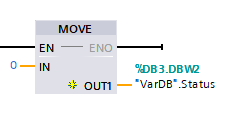
\includegraphics[width=0.4\textwidth]{Images/Chap3/move_block.png}
    \caption{A typical MOVE block in Ladder Diagram.}
    \label{fig:move_block_lad}
\end{figure}

\subsubsection{Set/Reset (SR) Blocks}
Functionality: The Set block forces a Boolean output to a TRUE state, while the Reset block forces it to a FALSE state.

When to Use: These blocks are used for direct control of output bits, such as a solenoid or a motor. The Set and Reset blocks for controlling outputs are shown in Figure \ref{fig:set_reset_blocks}. The two images show how an output can be Set or Reset to control the state of the Storage Cylinder.

 \begin{figure}[H]
    \centering
    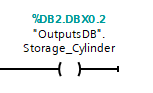
\includegraphics[width=0.3\textwidth]{Images/Chap3/set_block.png}
    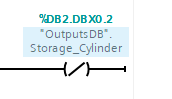
\includegraphics[width=0.31\textwidth]{Images/Chap3/reset_block.png}
    \caption{Set and Reset blocks for controlling outputs.}
    \label{fig:set_reset_blocks}
\end{figure}



\subsubsection{SR Flip-Flop}
Functionality: The SR (Set/Reset) flip-flop is a memory element. When the S input is activated, the output Q is set to TRUE. It remains TRUE even if the S input deactivates. The output is only reset to FALSE when the R input is activated. If both inputs are active at the same time, the R input has priority. The block for this logic is shown in \textbf{Figure \ref{fig:sr_flip_flop}}.

Inputs and Outputs: It has two Boolean inputs, S (Set) and R1 (Reset), and a single Boolean output, Q.

When to Use: This block is fundamental for implementing sequential logic. It is used to activate and hold the state of a step in the GRAFCET sequence until a new transition condition is met, such as setting the X\#3 bit to TRUE and holding it until the next step is ready.

\begin{figure}[H]
\centering
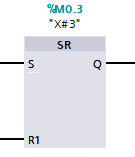
\includegraphics[width=0.2\textwidth]{Images/Chap3/sr_flip_flop.png}
\caption{The SR flip-flop block for sequential logic.}
\label{fig:sr_flip_flop}
\end{figure}

\subsubsection{Single-Shot Pulse (P\_TRIG)}
The P\_TRIG block generates a one-scan pulse on the rising edge of its input signal. This is crucial for triggering an action only once when a condition becomes true, preventing continuous execution that could lead to unexpected behavior. The P\_TRIG block is shown in \textbf{Figure \ref{fig:p_trig}}.
\begin{figure}[H]
\centering
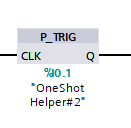
\includegraphics[width=0.2\textwidth]{Images/Chap3/trig.png}
\caption{The P\_TRIG block for single-scan pulses.}
\label{fig:p_trig}
\end{figure}
\subsection{Subroutines}
To simplify the main program loop and promote code reusability, several key functions were developed. These subroutines encapsulate specific, repeating logic, allowing the Main block to be a high-level overview of the entire process. This modular approach significantly improves readability, reduces the chance of errors, and makes the program easier to modify in the future. The process of adding a function block in TIA Portal is shown in \textbf{Figure \ref{fig:function_block}}.
\begin{figure}[H]
\centering
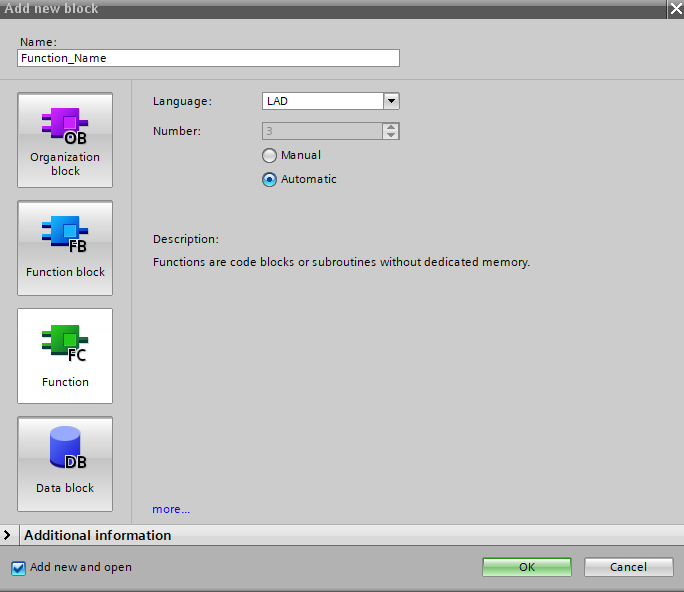
\includegraphics[width=0.5\textwidth]{Images/Chap3/Function.png}
\caption{Adding a function block in TIA Portal.}
\label{fig:function_block}
\end{figure}
\begin{itemize}
\item The DefaultState Function (FC2):
The DefaultState function is a crucial subroutine that ensures all key variables and outputs are reset to a safe, initial state. This function is called at the beginning of the program's Resetting Mode and whenever a cycle needs to be restarted. Its purpose is to guarantee a consistent and predictable starting point for every run, which is fundamental for system reliability and safety.

This function uses a series of MOVE blocks to set the values of the main state variables to their default safe values. As shown in \textbf{Figure \ref{fig:defaultstate}}, this includes resetting the Guide State, Gripper State, Robot Status, and Cube Color to a safe, initial value.

\begin{figure}[H]
    \centering
    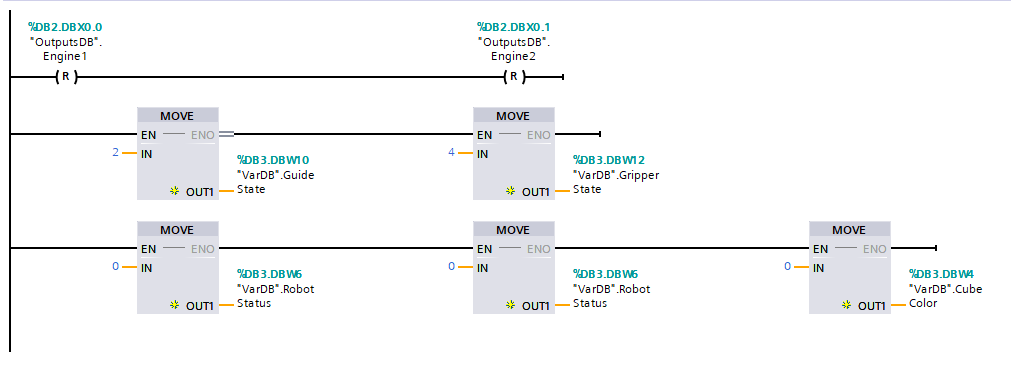
\includegraphics[width=0.9\textwidth]{Images/Chap3/DefaultState.png}
    \caption{Ladder logic for the DefaultState function.}
    \label{fig:defaultstate}
\end{figure}

\item The ResetOuts Function (FC1)
The ResetOuts function is a dedicated subroutine for turning off all outputs. It is called at the end of a cycle or when a fault is detected to ensure that no actuators are left active. This is a critical safety measure that prevents unintended movements or actions.

The function uses MOVE blocks to set the outputs to 0, effectively deactivating them. \textbf{Figure \ref{fig:resetouts}} shows this function resetting outputs for the motors, storage cylinder, gripper, and guide cylinder. The separation of this logic into a dedicated function ensures that the process of shutting down the system is both thorough and easy to manage from anywhere in the main program.

    \begin{figure}[H]
        \centering
        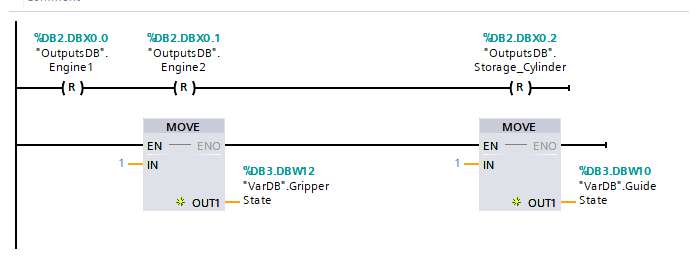
\includegraphics[width=1\textwidth]{Images/Chap3/ResetOuts.png}
        \caption{Ladder logic for the ResetOuts function.}
        \label{fig:resetouts}
    \end{figure}
\end{itemize}

\subsection{Sequential and Actuator Logic}
The core of the program is divided into input logic, which handles step transitions, and output logic, which controls actuators based on the current step. This separation simplifies development and debugging.

The input logic is the engine of the sequential program, with each transition represented by a separate network. As shown in \textbf{Figure \ref{fig:move_block_new}}, an SR flip-flop advances the program from the initial state (X\#0) to the next (X\#1). The flip-flop is set when the start button is pressed in the initial state and reset by the stop button or by advancing to a new step. Once set, a Move block writes the new step number to VarDB.Step.
\begin{figure}[H]
\centering
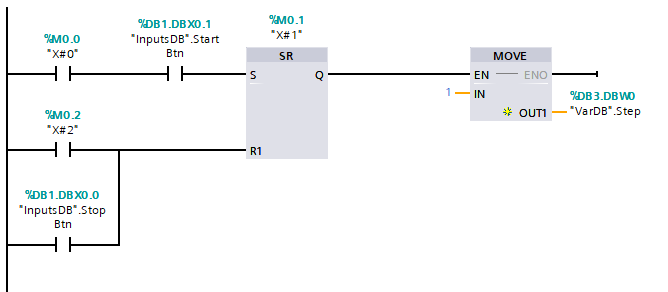
\includegraphics[width=1\textwidth]{Images/Chap3/network1.png}
\caption{Initial step logic with an SR flip-flop and a Move block.}
\label{fig:move_block_new}
\end{figure}

The output logic is straightforward. For each actuator, a dedicated network controls its state. \textbf{Figure \ref{fig:storage_cylinder_logic}} shows the logic for the Storage Cylinder, which extends when the program is in step (X\#1) and the status is set to Running (VarDB.Status = 1).
\begin{figure}[H]
\centering
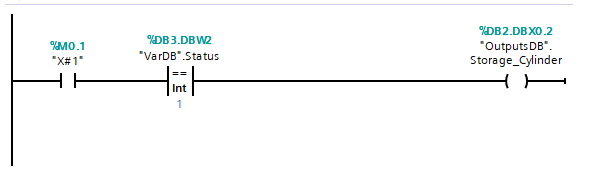
\includegraphics[width=1\textwidth]{Images/Chap3/network17.png}
\caption{Sample output logic for the Storage Cylinder.}
\label{fig:storage_cylinder_logic}
\end{figure}

The logic for returning the system to its initial state is shown in \textbf{Figure \ref{fig:tags_steps_home}}. This network is responsible for a complete system reset based on sensor checks. An SR flip-flop is used to manage this state. Its set input is activated by a combination of the (X\#1) step being active and all sensors confirming that the cylinders are in their home positions. Once these conditions are met, a Move block writes the value 0 to VarDB.Step, returning the system to the initial state (X\#0). The flip-flop is reset only by the (X#1) step, ensuring the system can be automatically reset.
\begin{figure}[H]
\centering
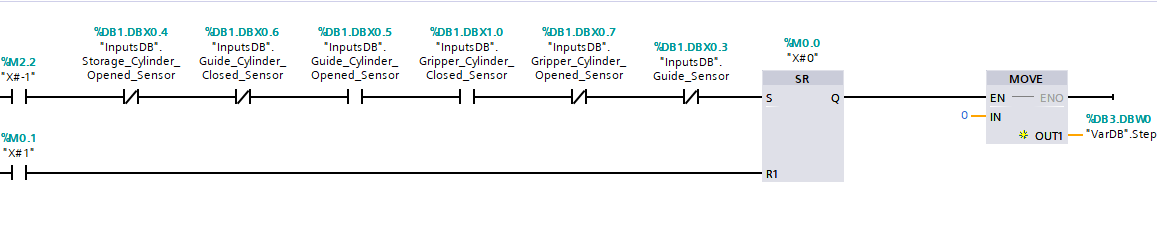
\includegraphics[width=1\textwidth]{Images/Chap3/network21.png}
\caption{Transition logic for resetting the system to the home position.}
\label{fig:tags_steps_home}
\end{figure}

More complex logic, such as sending commands to the KUKA robot, is handled by a single-shot pulse. As shown in \textbf{Figure \ref{fig:robot_logic}}, a P\_TRIG block is triggered once when the system enters step (X\#7) and the VarDB.Status is 1. This pulse then triggers a sequence of three Move blocks to command the robot's position and gripper state.
\begin{figure}[H]
\centering
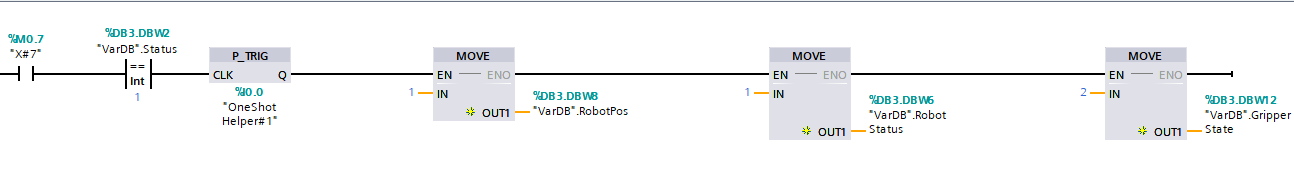
\includegraphics[width=1\textwidth]{Images/Chap3/network111.png}
\caption{Logic for sending commands to the KUKA robot.}
\label{fig:robot_logic}
\end{figure}

The logic for the guide cylinder, shown in \textbf{Figure \ref{fig:guide_cylinder_logic}}, operates with three distinct states controlled by VarDB.GuideState: 1 for idle, 2 for extend, and 4 for close. The logic incorporates sensor checks to prevent over-extension or over-retraction. This same logic, with minor adjustments for specific sensor and actuator tags, is also used for the gripper cylinder.
\begin{figure}[H]
\centering
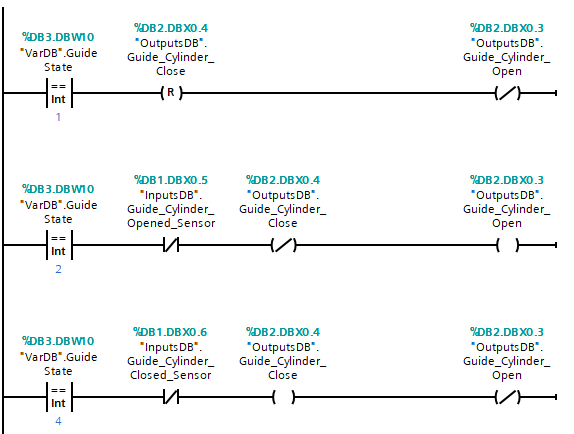
\includegraphics[width=0.8\textwidth]{Images/Chap3/network_guide_cylinder_logic1.png}
\caption{Logic for controlling the guide cylinder.}
\label{fig:guide_cylinder_logic}
\end{figure}

The last main block of logic handles the sorting process, as shown in \textbf{Figure \ref{fig:sorting_logic}}. When the system is in Running mode (VarDB.Status = 1) and VarDB.Step is equal to 9, a single pulse is generated by the P\_TRIG block. The first Move block then writes 1 to VarDB.RobotStatus, indicating the robot is ready to move to the pick-up position. A series of conditional branches then check the value of VarDB.CubeColor. Based on the color (1 for red, 2 for green, 3 for blue), a Move block commands the robot to move to the correct sorting position and a counter for that color is incremented.
\begin{figure}[H]
\centering
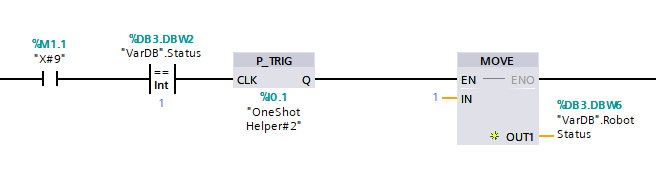
\includegraphics[width=0.8\textwidth]{Images/Chap3/network_sorting_logic1.png}
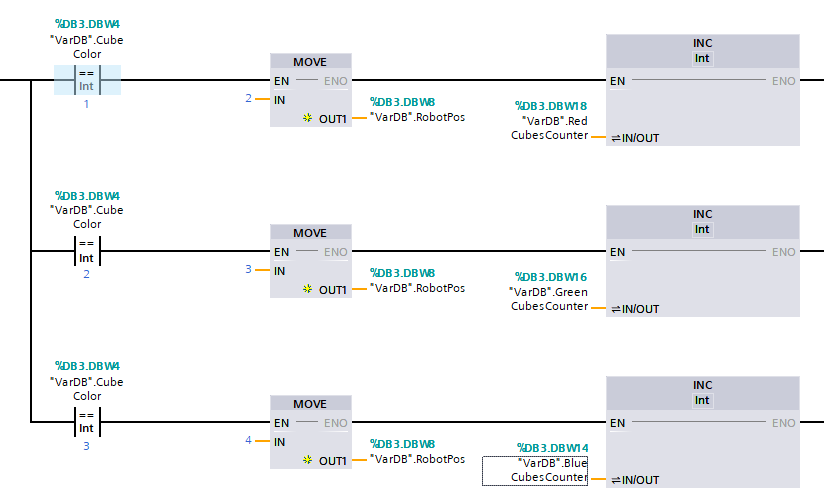
\includegraphics[width=0.8\textwidth]{Images/Chap3/network_sorting_logic2.png}
\caption{Logic for the sorting process.}
\label{fig:sorting_logic}
\end{figure}

\section{HMI Programming and Design}
This section focuses on the development of the Human-Machine Interface (HMI) using the TIA Portal framework. It will cover the creation of graphical user interface screens, the design of interactive elements like buttons and indicators, and the configuration of communication links to the PLC.

\subsection{Screen Navigation and Layout}
This section will detail the purpose and layout of the two main screens that were designed for system operation and maintenance.

\subsubsection{Production Screen}
The Production Screen serves as the primary operational interface for the sorting cell. Its design is focused on providing the operator with a clear and concise overview of the machine's status and real-time production data. The screen layout is intuitive, with key control buttons and status indicators located in a central position.

As shown in \textbf{Figure \ref{fig:production_screen}}, the screen includes:
\begin{itemize}
\item Cube Counters: Three distinct counters display the total number of red, blue, and green cubes sorted. These counters are linked to integer tags in the PLC and update in real-time, providing immediate feedback on the sorting process;
\item Status Indicators: The "Machine Status" and "Robot Status" boxes provide a visual indication of the system's current state. The text and color of these boxes change dynamically based on the corresponding integer values from the PLC, allowing the operator to quickly assess the machine's condition;
\item Control Buttons: Large, clearly labeled buttons for "Start," "Stop," and "Pause" allow the operator to control the main operational cycle. A key safety feature implemented is that these buttons are only enabled or disabled based on the machine's current state. For example, the "Start" button is only accessible when the machine is in the Stop or Pause mode, preventing accidental activation.
\end{itemize}
The "Maintenance" button provides a direct navigation link to the dedicated maintenance screen.

\begin{figure}[H]
\centering
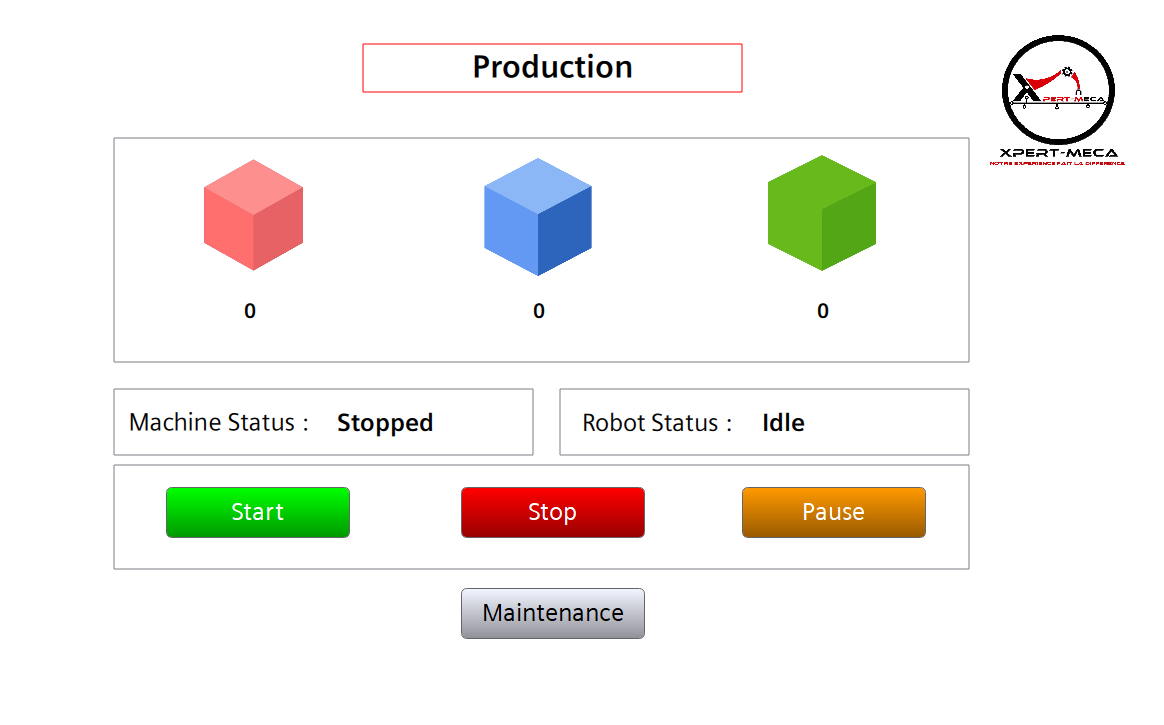
\includegraphics[width=0.8\textwidth]{Images/Chap3/production_screen.png}
\caption{The Production Screen of the HMI.}
\label{fig:production_screen}

\end{figure}

\subsubsection{Maintenance Screen}
The Maintenance Screen is a dedicated interface for troubleshooting, manual control, and detailed diagnostics. Unlike the Production Screen, which is designed for quick operation, the Maintenance Screen provides a comprehensive overview of the system's internal state and allows the operator to manually override outputs and simulate inputs. This mode is critical for commissioning and debugging the system. The overall layout is shown in \textbf{Figure \ref{fig:maintenance_screen}}.

The screen is organized into distinct functional areas:
\begin{itemize}
\item Status Display: This section provides granular, real-time status information, including the "Machine State," "Robot State," "Current Step" in the PLC program, and the "Cube Color" detected by the vision system;
\item Input Simulation Buttons: A key feature is the ability to manually trigger simulated inputs. This array of buttons, corresponding to physical sensors (e.g., "End of Road Sensor") and start/stop buttons, allows technicians to test the PLC logic without requiring the physical presence of parts or the activation of real-world sensors;
\item Output Visualization and Control: This area provides a visual representation of the system's key outputs. The operator can see the status of motors and cylinders and, crucially, can manually control them by toggling switches and pressing buttons to diagnose issues or perform manual maneuvers.
\end{itemize}
The "Back" button at the top left allows for seamless navigation back to the Production screen.

\begin{figure}[H]
\centering
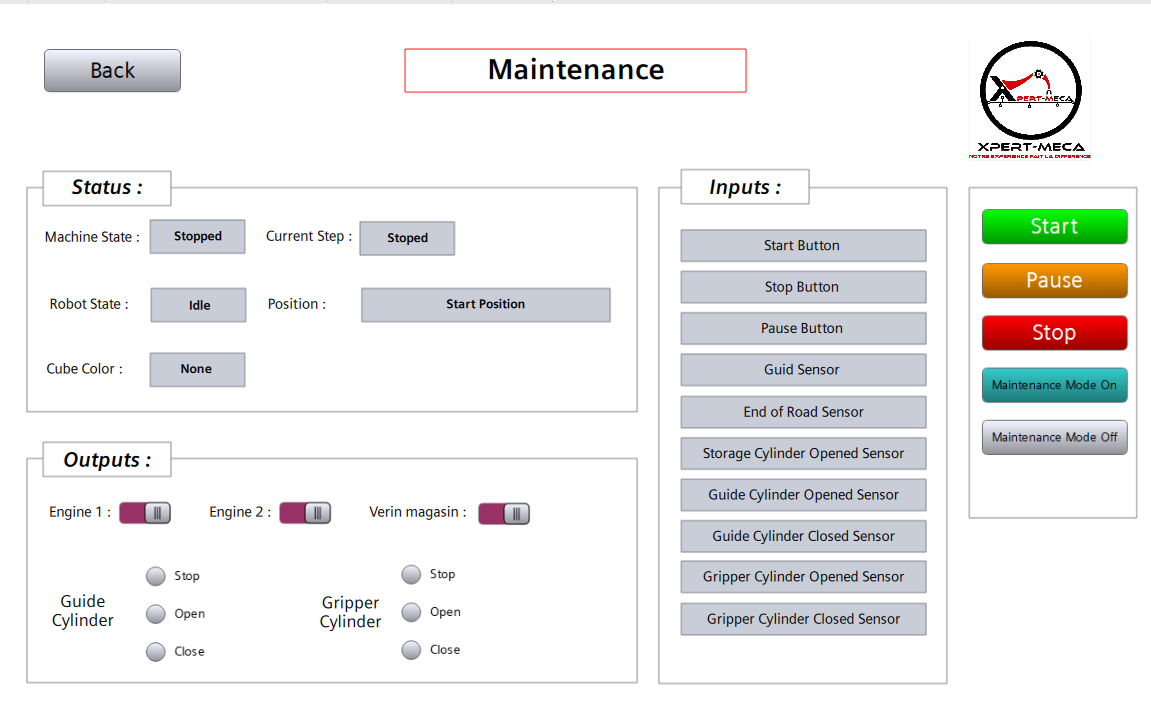
\includegraphics[width=1\textwidth]{Images/Chap3/maintenance_screen.png}
\caption{The Maintenance Screen of the HMI.}
\label{fig:maintenance_screen}
\end{figure}


\subsection{Dynamic Status Indicators}
The status indicators on the HMI screens are not static, they change their text and color based on the machine’s real-time state. This dynamic feedback is crucial for providing operators with immediate visual cues. This effect is achieved by linking the display element's properties to a PLC tag and configuring a range of values.

\subsubsection{Linking a Variable to a Text String}
This process allows a numerical value from the PLC to be displayed as descriptive text on the HMI. For example, a PLC variable with the value 1 can be shown as "RUNNING."

\begin{enumerate}
\item Create the Text List: In the HMI project tree in TIA Portal, navigate to HMI Tags Text and graphic lists and add a new list. This is the central repository for defining the text associated with each value.
\item Define List Entries: In the new text list, add entries for each state. Each entry requires a value and a corresponding text string. For the "Machine Status" indicator, we would define entries such as:
\begin{itemize}
\item Value 0: Text "Stopped";
\item Value 1: Text "Running";
\item Value 2: Text "Paused";
\item Value 3: Text "Maintenance";
\item Value 4: Text "Resetting".
\end{itemize}
\textbf{Figure \ref{fig:status_text}} shows how this is configured in TIA Portal.
\begin{figure}[H]
\centering
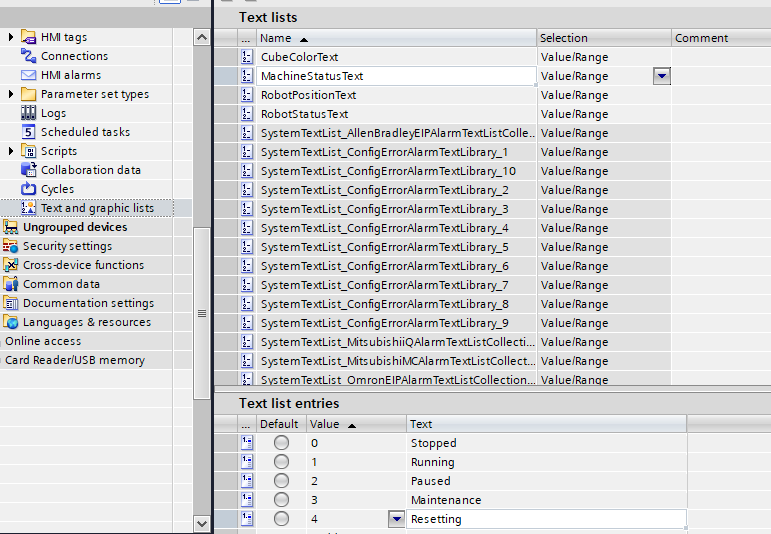
\includegraphics[width=0.8\textwidth]{Images/Chap3/status_text.png}
\caption{HMI configuration for a status text list that links a variable's value to a text string.}
\label{fig:status_text}
\end{figure}
\item Link the Text Box: On the HMI screen, place a text box or an I/O field. In its properties, navigate to General > Text and link it to the PLC tag that represents the machine's status (e.g., VarDB.MachineStatus). Then, under Text list, select the list you just created. The HMI will now automatically display the correct text based on the tag's current value. \textbf{Figure \ref{fig:text_list_link}} shows how to link the text box to the PLC variable.
\begin{figure}[H]
\centering
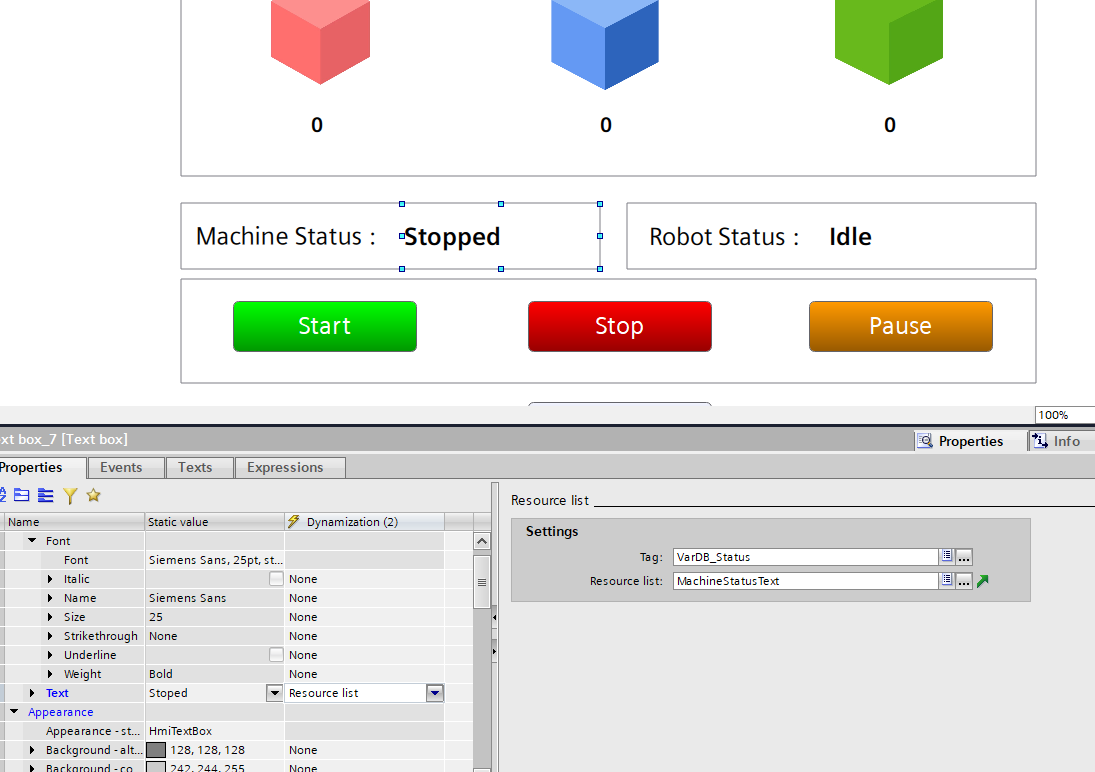
\includegraphics[width=1\textwidth]{Images/Chap3/link.png}
\caption{HMI properties panel for linking a text box to a PLC variable and a text list.}
\label{fig:text_list_link}
\end{figure}
\end{enumerate}

\subsubsection{Linking a Variable to a Color}
To make the status indicator even more intuitive, its background color can change dynamically to reflect the machine's state (e.g., red for STOPPED, green for RUNNING, orange for PAUSED, blue for MAINTENANCE and yellow for RESETTING).

\begin{enumerate}
\item Add a Graphic Element: Place a basic shape, such as a rectangle, on the HMI screen. This will serve as the background for the status text.
\item Configure Animations: In the properties of the graphic element, navigate to Animations and add a new animation of type Appearance.
\item Link to the PLC Tag: In the animation configuration, link the graphic to the same PLC tag used for the text list (VarDB.MachineStatus).
\item Set the Color Ranges: Define the color for each possible value of the tag. For example:
\begin{itemize}
\item Value 0: Background color is set to Red;
\item Value 1: Background color is set to Green;
\item Value 2: Background color is set to Orange;
\item Value 3: Background color is set to Blue;
\item Value 4: Background color is set to Yellow.

\end{itemize}
This is visually configured by setting the ranges, as seen in Figure \ref{fig:status_color_config}.
\begin{figure}[H]
    \centering
    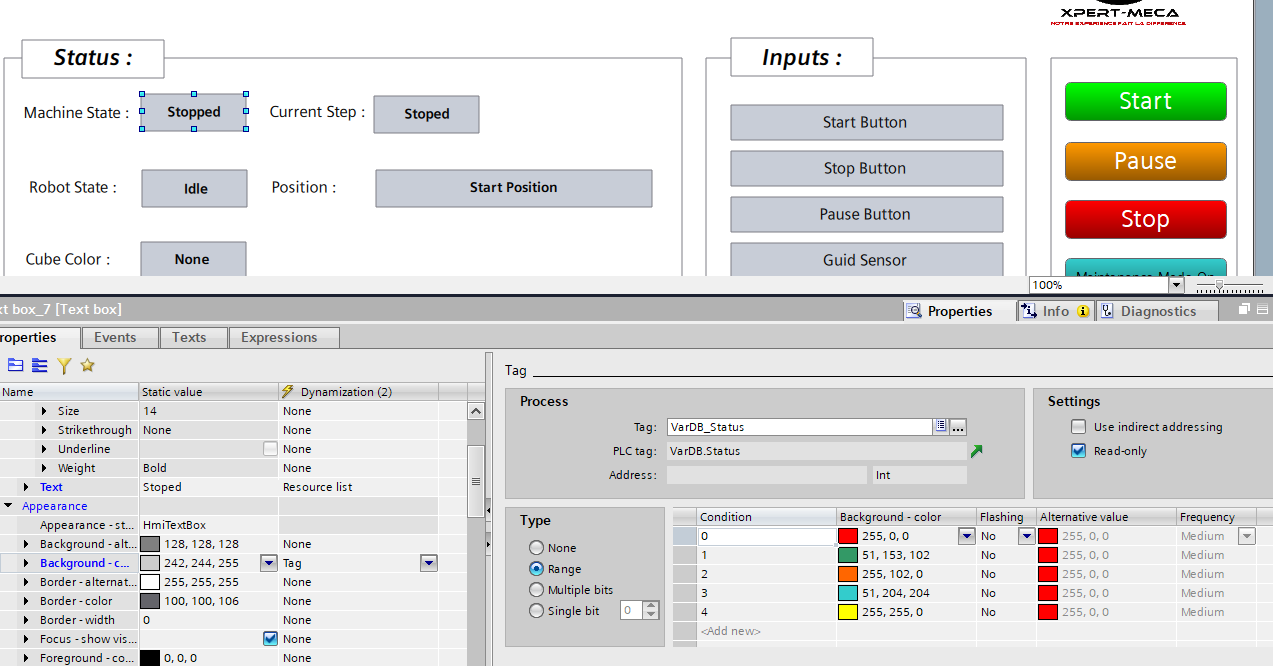
\includegraphics[width=1\textwidth]{Images/Chap3/_color.png}
    \caption{HMI configuration for changing an element's background color based on a variable's value.}
    \label{fig:status_color_config}
\end{figure}
\item Final Placement: Place the text box from the previous step on top of this graphic element. The result is a single status indicator that changes both its text and background color dynamically, as shown in Figure \ref{fig:status_color}.

\end{enumerate}

\begin{figure}[H]
    \centering
    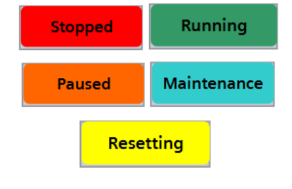
\includegraphics[width=0.5\textwidth]{Images/Chap3/state_boxes.png}
    \caption{Visual result of a status box with dynamic text and color.}
    \label{fig:status_color}
\end{figure}

\subsection{Dynamic Control and Button Interactivity}
The control buttons ("Start," "Stop," "Pause") are also configured to be interactive, preventing erroneous operations and enhancing safety. They are enabled or disabled based on the PLC’s status.

\begin{enumerate}
\item Add the Button: Place a button element on the HMI screen and give it a descriptive name like "Start\_Button."
\item Configure the Button's Event: In the button's properties, go to Events > Press. This is where you define the action the button will perform. For the "Start" button, the event uses a "SetTagValue" function to write the value 1 to the InputsDB\_StartBtn bit in the PLC, as shown in Figure \ref{fig:button_event}.
\begin{figure}[H]
\centering
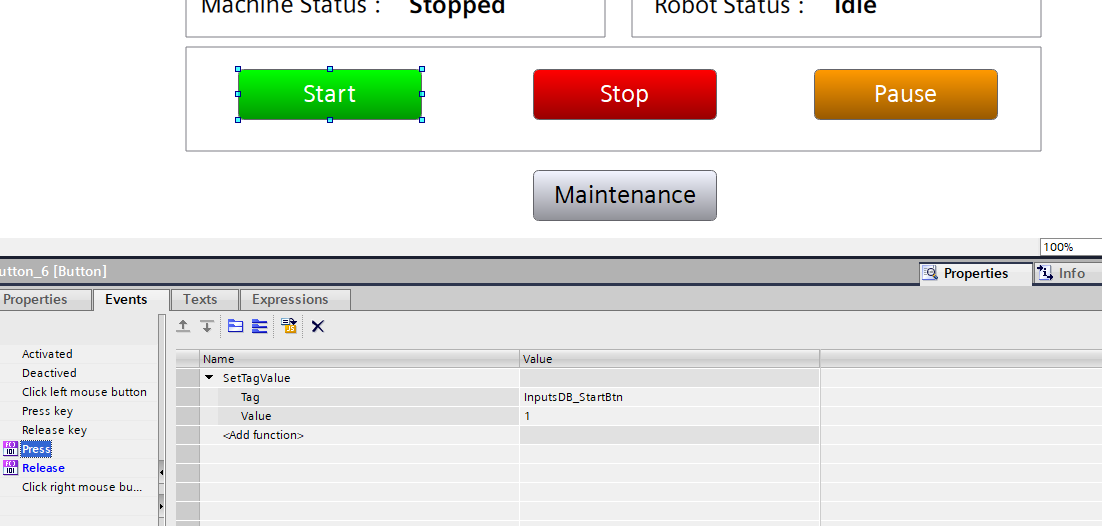
\includegraphics[width=1\textwidth]{Images/Chap3/_event.png}
\caption{HMI event configuration for a button press, which sets a PLC tag.}
\label{fig:button_event}
\end{figure}
\item Configure Button Operability: To control when the button can be pressed, navigate to the Properties of the button and go to General > Operability. Link this property to the PLC status tag (VarDB.MachineStatus). Then, configure the range so that the "Start" button is only operable when the MachineStatus tag is equal to 0 or 2 (the "STOPPED" or "PAUSED" state). This prevents the machine from being started while it is already running. The configuration is shown in Figure \ref{fig:button_operability_config}, and examples of multiple operability cases for buttons are shown in Figure \ref{fig:button_operability}.
\begin{figure}[H]
\centering
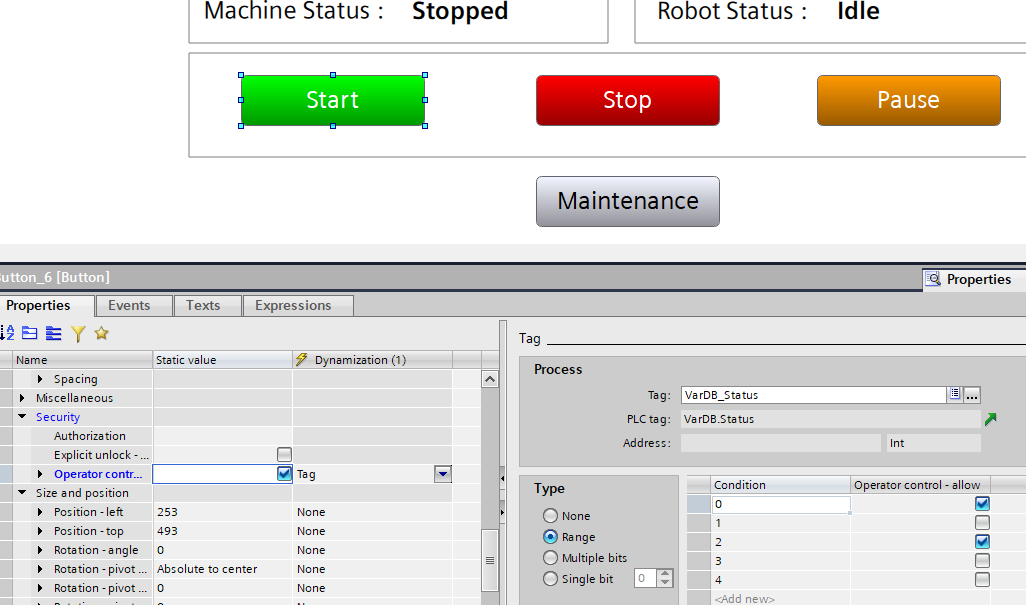
\includegraphics[width=0.8\textwidth]{Images/Chap3/_operability.png}
\caption{HMI configuration to link a button's operability to a PLC variable.}
\label{fig:button_operability_config}
\end{figure}
\end{enumerate}
\begin{figure}[H]
\centering
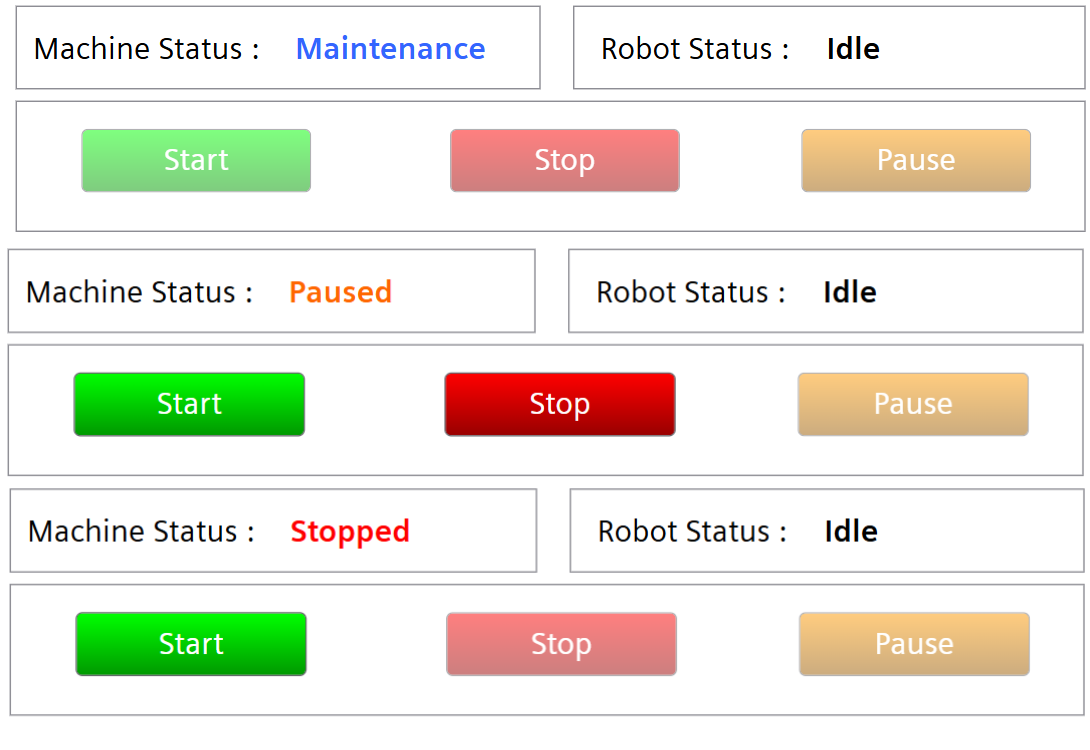
\includegraphics[width=0.6\textwidth]{Images/Chap3/MULTIPLECASES.png}
\caption{Examples of multiple operability cases for buttons.}
\label{fig:button_operability}
\end{figure}
\subsection{Real-time Value Displays (Counters)}
A critical function of the HMI is to provide real-time data to the operator, such as the count of sorted cubes.

\begin{enumerate}
\item Add a Display Field: Place an I/O field or a simple text box on the HMI screen.
\item Link to the PLC Tag: In the properties of the display field, navigate to General and link the Process value to the corresponding integer tag in the PLC (e.g., VarDB.RedCubesCounter), as shown in Figure \ref{fig:value_displays_config}.
\begin{figure}[H]
\centering
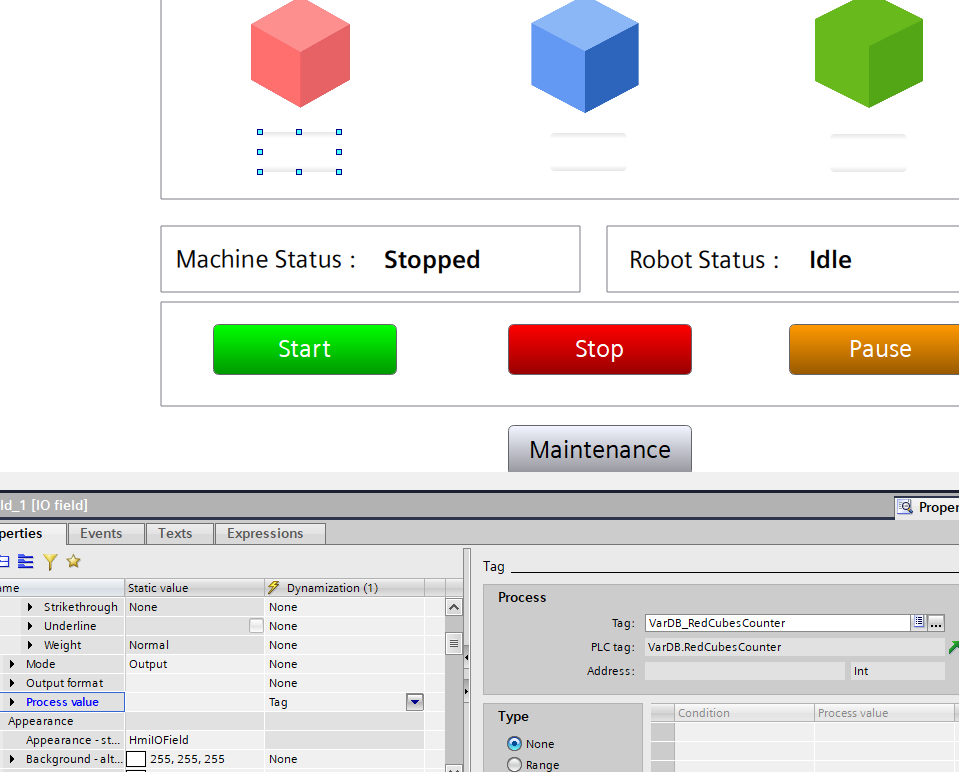
\includegraphics[width=0.8\textwidth]{Images/Chap3/value_displays.png}
\caption{HMI configuration for linking a display element to an integer tag in the PLC.}
\label{fig:value_displays_config}
\end{figure}
\item Format the Display: Configure the display format (e.g., number of decimal places, font, size) as needed. As the PLC tag's value increments, the number displayed on the HMI screen will update in real-time. The real-time display of cube counters on the HMI is shown in Figure \ref{fig:value_displays}.
\end{enumerate}
\begin{figure}[H]
\centering
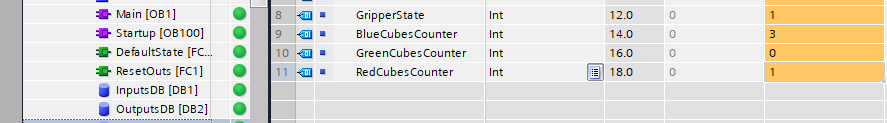
\includegraphics[width=0.8\textwidth]{Images/Chap3/cubecounters_vardb.png}
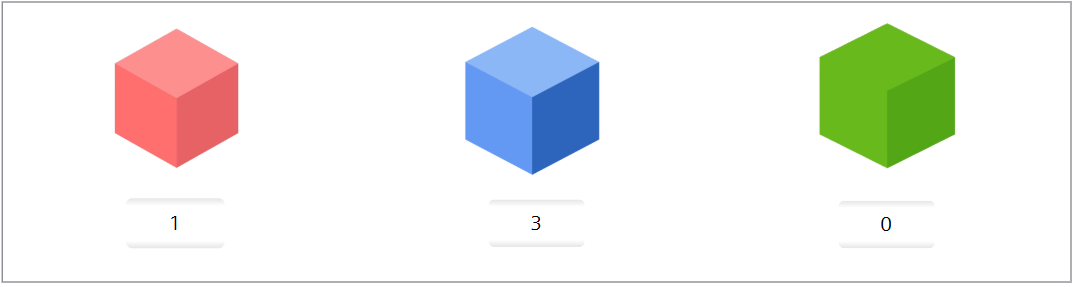
\includegraphics[width=0.8\textwidth]{Images/Chap3/cubecounters_hmi.png}
\caption{Real-time display of cube counters on the HMI.}
\label{fig:value_displays}
\end{figure}






\section{Conclusion}
The implementation of the control system for the robotic sorting cell, as detailed in this chapter, provides a comprehensive overview of the automation and human-machine interface development. We established a robust control philosophy centered on a Programmable Logic Controller (PLC) and utilized GRAFCET to meticulously design the sequential logic. While the complete, exhaustive programming of the automation and HMI is extensive, this chapter has presented the most critical and foundational steps. The provided logic blocks, programming principles, and design methods for elements like real-time counters and button operability are all that are necessary to construct the entire functional and structured control system. Crucially, the system's design also prioritizes the safety of the cell's operation and personnel, ensuring a secure and reliable sorting process. The structured approach outlined here is the cornerstone of a predictable, efficient, and safe robotic sorting solution.






















